\documentclass[a4paper, 11pt]{article}
\usepackage{comment} % enables the use of multi-line comments (\ifx \fi) 
\usepackage{lipsum} %This package just generates Lorem Ipsum filler text. 
\usepackage{fullpage} % changes the margin

\usepackage[T1]{fontenc}
\usepackage[english]{babel}
\usepackage[utf8]{inputenc}
\usepackage{lmodern}
\selectlanguage{english}
\usepackage{graphicx}
\usepackage{float}



\begin{document}
\noindent
\large\textbf{Post-Lab Multiscale Report} \hfill \textbf{Krzysztof Belcarz} \\
 \hfill Raport Date: 13/11/18 

\section*{Graphical User Interface}
Program's graphical user interface looks as follows:
\begin{figure}[H]
\centering
  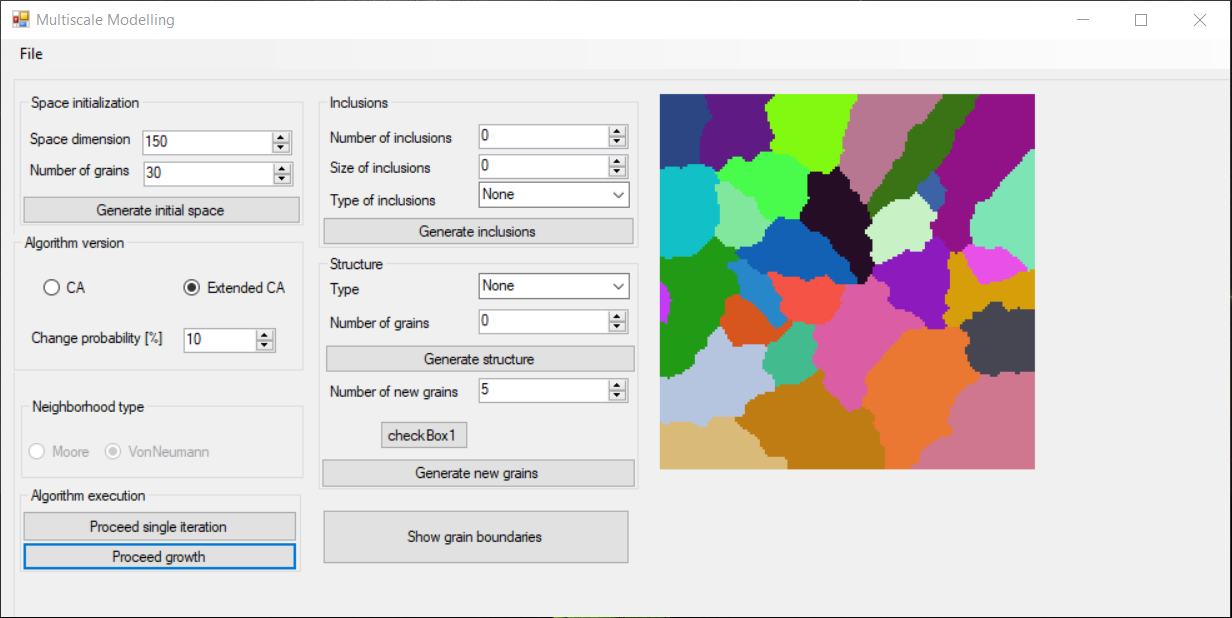
\includegraphics[width=\linewidth]{GUI}
  \caption{GUI}
  \label{fig:boat1}
\end{figure}
In order to proceed with any algorithm one needs to generate space of desired size with inputted number of grains:
\begin{figure}[H]
\centering
  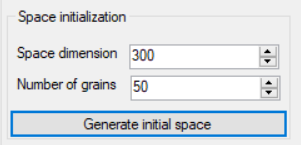
\includegraphics{SpaceInit}
  \caption{Space initialization group box}
  \label{fig:boat1}
\end{figure}
\section*{Class 1 - Simple grain growth}
During first class the task was to implement basic version of Cellular Automata algorithm with utilizing classic Moore and VonNeumann neighborhood types. In order to ensure correct algorithm operation absorbing boundary condition was introduced. The state of cells on the edges of solution space were fixed with a specific value (0 in particular), thus they are not taken into account when updating grain structure.

In algorithm version group box \textbf{CA} radio button must be checked:
\begin{figure}[H]
\centering
  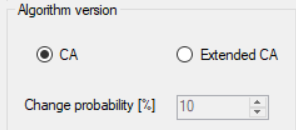
\includegraphics{SimpleCAGroupBox}
  \caption{Simple CA}
  \label{fig:boat1}
\end{figure}

After the growth utilizing simple CA is complete a space such as the one presented below is produced.
\begin{figure}[H]
\centering
  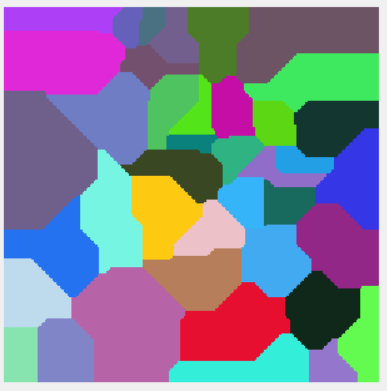
\includegraphics[]{SimpleCAExample}
  \caption{Example of simple CA algorithm}
  \label{fig:boat1}
\end{figure}


\section*{Class 2 - Microstructure import/export}
Second class goal was to implement mechanism of importing/exporting grain structure from/to file. In order to do so one shall access \textbf{File->Export data} or \textbf{File->Import data} depending on intentions.
\begin{figure}[H]
\centering
  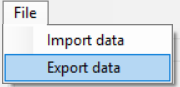
\includegraphics{File}
  \caption{Import/export menu}
  \label{fig:boat1}
\end{figure}
\subsection{Exporting state}
State is saved simultaneusly in a bitmap and in a text file. User is able to choose the location where the files are supposed to be stored. Name for each file is generated automatically and is unique, because of the fact that it includes current date.

\begin{figure}[H]
\centering
  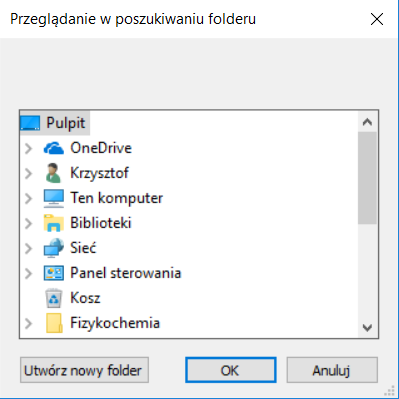
\includegraphics[]{ExportTo}
  \caption{Export dialog}
  \label{fig:boat1}
\end{figure}

\subsubsection{Exporting state to bitmap}
\subsubsection{Exporting state to .txt file}

\subsection{Importing state}

\begin{figure}[H]
\centering
  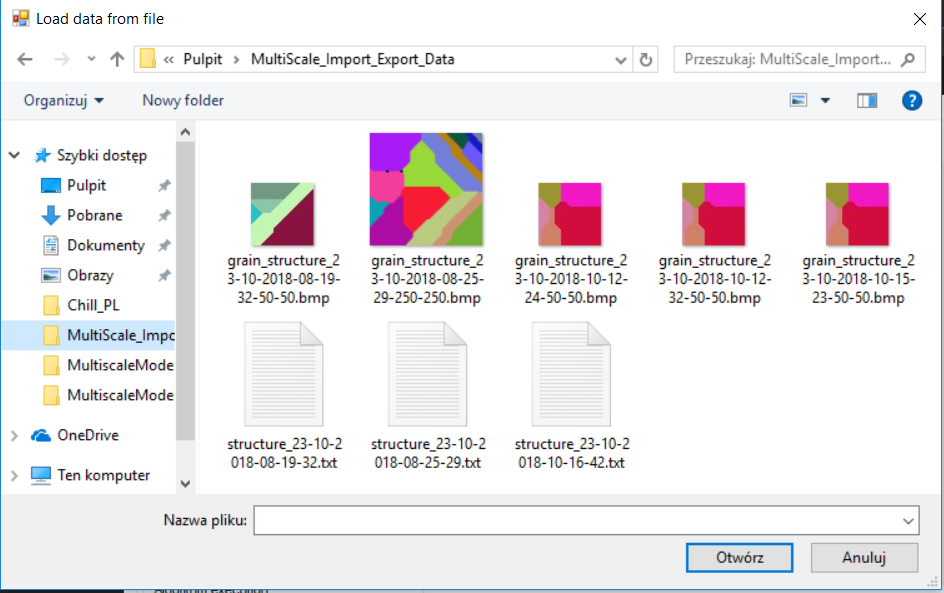
\includegraphics[width=\linewidth]{ImportFrom}
  \caption{Import dialog}
  \label{fig:boat1}
\end{figure}

\subsubsection{Importing state from .txt file}
The format of txt file is as follows:
\begin{enumerate}
\item Dimension of space
\item Header
\item Values corresponding to header's columns
\end{enumerate}
Example of such file:
\begin{figure}[H]
\centering
  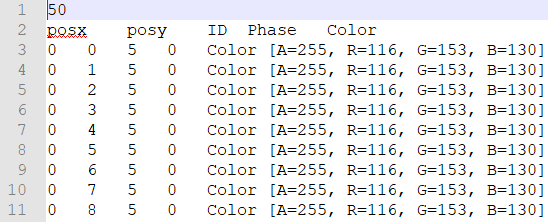
\includegraphics[]{ExportedTxt}
  \caption{structure$\_$23-10-2018-08-19-32.txt}
  \label{fig:boat1}
\end{figure}
\subsubsection{Importing state from bitmap}
\begin{figure}[H]
\centering
  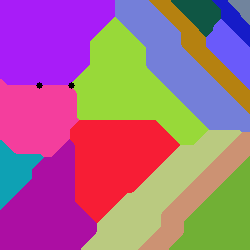
\includegraphics[]{ExportedBitmap}
  \caption{grain$\_$structure$\_$23-10-2018-08-25-29-250-250.bmp}
  \label{fig:boat1}
\end{figure}

\section*{Class 3 - Inclusions}
Aim of next class was to introduce a feature which would allow user to add inclusions to grain structure either before the growth (in any place/coordinates) or after the growth (only on grain borders).
Inclusions are defined with following parameters:
\begin{itemize}
\item number - how many inclusions to create
\item size - what is the diameter (circular)/ side (square) of a single inclusion
\item type - what type of inclusions to create (circular/square)
\end{itemize}
A callback function is connected to structure display space, so that user can click and add inclusions of his/her choosing before the growth starts and a dedicated button is responsible for generating inclusions specified with parameters in corresponding group box is also available.\newline
Any action will take place only when type of inclusion is changed to a valid one (from default None) and automatic generation will take place only when number of inclusions is positive, as well as, their size.
\begin{figure}[H]
\centering
  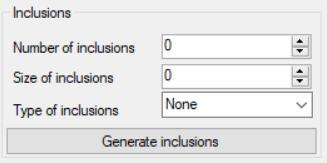
\includegraphics[]{InclusionsGroupBox}
  \caption{Inclusions group box}
  \label{fig:boat1}
\end{figure}


Example of structure with circular inclusions:
\begin{figure}[H]
\centering
  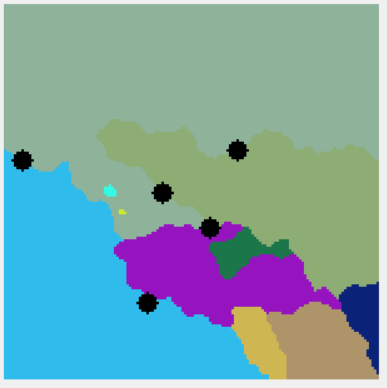
\includegraphics[]{CircularInclusionsExample}
  \caption{Example of circular inclusions}
  \label{fig:boat1}
\end{figure}

Example of structure with square inclusions:
\begin{figure}[H]
\centering
  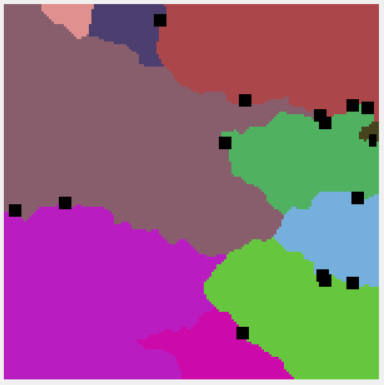
\includegraphics[]{SquareInclusionsExample}
  \caption{Example of square inclusions}
  \label{fig:boat1}
\end{figure}
\section*{Class 4 - Extended CA}
Fourth class purpose was to implement extended version of Cellular Automata algorithm. Instead of one rule used in basic four rules were implemented, featuring new types of neighborhoods, as well as, new conditions for changing state of a particular cell.

In order to take adventage of extended version of the algorithm it must be checked on algorithm version group box:
\begin{figure}[H]
\centering
  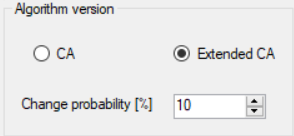
\includegraphics{ExtendedCAGroupBox}
  \caption{Extended CA}
  \label{fig:boat1}
\end{figure}
Then and only then probability parameter for 4th rule is unlocked for modification.

After the growth utilizing extended CA is complete a space such as the one presented below is produced.
\begin{figure}[H]
\centering
  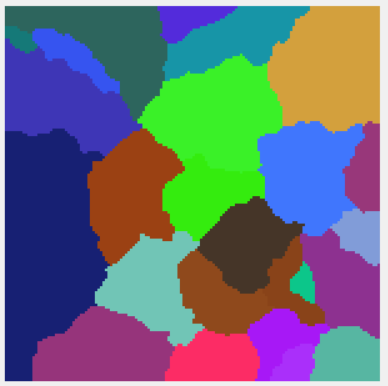
\includegraphics[]{ExtendedCAExample}
  \caption{Example of extended CA algorithm}
  \label{fig:boat1}
\end{figure}



\section*{Class 5 - Substructures/Dual phase}
In course of class number 5 we were supposed to give user possibility to create a substructure or dual phase after initial growth. User can choose how many grains from initial growth are meant to be considered while creating substructure of dual phase. After those grains are ''transformed'' according to user preference new grains can be added and once more growth is possible.
\subsection{Substructure}
User defined number of grains is preserved on the space with their original color and IDs.
\begin{figure}[H]
\centering
  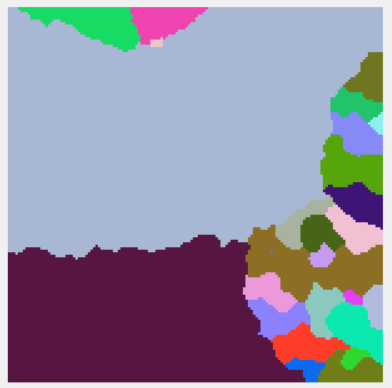
\includegraphics[]{SubstructureExample}
  \caption{Example of a substructur}
  \label{fig:boat1}
\end{figure}
\subsection{Dual phase}
User defined number of grains is preserved on the space with a new color common for all of them and their phase parameter is incremented.
\begin{figure}[H]
\centering
  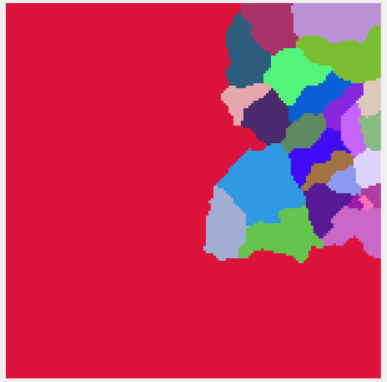
\includegraphics{DualPhaseExample}
  \caption{Example of dual phase}
  \label{fig:boat1}
\end{figure}
\section*{Class 6 - Grain boundaries}
After the growth with chosen algorithm version is complete user can generate grain boundaries and display them.
\begin{figure}[H]
\centering
  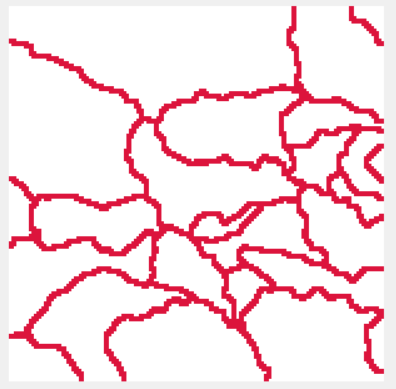
\includegraphics[]{GrainBoundariesExample}
  \caption{Example grain boundaries}
  \label{fig:boat1}
\end{figure}
\section*{Attachments}
%Make sure to change these
%Lab Notes, HelloWorld.ic, FooBar.ic
%\fi %comment me out

\begin{thebibliography}{9}
\bibitem{Robotics} Fred G. Martin \emph{Robotics Explorations: A Hands-On Introduction to Engineering}. New Jersey: Prentice Hall.
\bibitem{Flueck}  Flueck, Alexander J. 2005. \emph{ECE 100}[online]. Chicago: Illinois Institute of Technology, Electrical and Computer Engineering Department, 2005 [cited 30
August 2005]. Available from World Wide Web: (http://www.ece.iit.edu/~flueck/ece100).

%\bibitem{general_ElectricMobility} https://electricmobility.expert/poziomy-jazdy-autonomicznej-volvotalks-pojazdy-autonomiczne/ dostęp z dnia:
%\bibitem{general_SpidersWeb} https://www.spidersweb.pl/2016/07/samochod-autonomiczny.html dostęp z dnia:
%\bibitem{general_Chip} https://www.chip.pl/2017/09/dziala-autonomiczne-auta/ dostęp z dnia:

\end{thebibliography}

\end{document}
